\chapter{Implementace}

\section{Výběr technologií}

V době, kdy existuje obrovské množství programovacích jazyků, jejich ekosystémů a dalších frameworků je důležité se umět nespálit. 
Vybrat špatné technologie totiž může znamenat prodloužení vývoje, zvýšení celkových nákladů nebo dokonce ukončení projektu.
Proto je nutnost tuto část dostatečně analyzovat a svědomitě zvážit, aby nedošlo k omylu, který by zabraňoval úspěšné dokončení.
Pro adekvátní výběr tak bylo potřeba specifikovat příslušná kritéria, které by jasně porovnala všechny zvažované technologie:

\subsubsection*{Podpora webových služeb}
Při tvorbě webové aplikace nemůže být ani řeč o technologii, která by pro použití na webu nebyla vhodná. Technologie musí
umět pracovat s mapováním URL a HTTP metod na zdroje a pracovat s běžnými formáty dat v internetové komunikaci (např. JSON).

\subsubsection*{Dokumentace a uživatelská podpora}
Pro pochopení technologie a její správné používání je často potřeba znát detaily, které se uživatel dozví z dokumentace.
Ta dokáže často výrazně zkrátit učící křivku a programátorovi tak šetří čas. Pokud dokumentace nestačí, může často její
nedostatky zachránit dostatečně široká uživatelská základna. Velká uživatelská podpora navíc snižuje riziko zestárnutí zvolené technologie.

\subsubsection*{Znalost technologie}
Pokud již programátor některou z technologií zná, může mu tato znalost ušetřit mnoho času při vývoji. Nemusí totiž novou technologii
nijak složitě zavádět nebo se učit její použití. Vhodným výběrem se také může vyvarovat situacím, kdy až v průběhu implementace narazí
na neřešitelné problémy. Zavrhnout neznámé technologie ale může znamenat přijít o možnost používat nástroje, které jsou problémům šité na míru. 

\subsubsection*{Výkon}
I když aplikace nepočítá s vetším provozem čítající stovky požadavků za sekundu, není důvod používat technologie, které jsou pomalé
nebo spotřebovávají příliš moc prostředků.

\section{Zvolené technologie}

\subsection{Programovací jazyk Python}

Python\cite{python} je víceúčelový skriptovací jazyk navrhnut v roce 1991 \cite{python-year} Guido van Rossumem.
Je vyvíjen jako open source projekt a je bezplatně dostupný pro většinu dostupných platforem (Unix, Windows, Mac OS).
V distribucích Linuxu je často součástí základní instalace. Díky velkému množství knihovních modulů z různých oblastí
má velice široké možnosti uplatnění. Běžně jej používají ve firmách jako Google, Dropbox, YouTube, Red Hat, Cisco,
Facebook nebo Microsoft \cite{python-companies}.

Protože jde o dynamický interpretovaný jazyk, jeho zdrojový kód není nutné překládat překladačem do strojového kódu.
Je to zárovéň hybridní jazyk, protože umožňuje používat různá programovací paradigmata, včetně objektově orientovaného,
imperativního, procedurálního nebo v omezené míře i funkcionálního. I když je Python mnohokrát označován za skriptovací jazyk,
jeho návrh umožňuje psaní rozsáhlých a plnohodnotných aplikací včetně GUI. Podporuje také dynamickou kontrolu datových typů.

Je to jazyk, který se velmi snadno učí a bývá považován za jeden z nejvhodnějších programovacích jazyků pro začátečníky.
Pomáhá tomu jeho jednoduchá syntaxe a čistota kódu. Na rozdíl od jiných jazyků bývá jeho zdrojový kód často krátký a dobře čitelný.
Je tak vhodný pro výuku i využití v praxi. Podle PYPL indexu\footnote{PopularitY of Programming Language Index je vytvořen analyzováním toho,
jak často jsou tutoriály jednotlivých programovacích jazyků hledány na Googlu.} je Python celosvětově nejrychleji roustoucí programovací jazyk
v~oblíbenosti za posledních pět let \cite{python-pypl} a v jeho dubnovém žebříčku roku 2016 drží druhé místo mezi jazyky Java a PHP.
Mnoho dalších žebříčků pak uvádí Python vždy v prvních pěti místech.

Po stránce výkonu je na tom Python relativně dobře, protože mnoho na~výkon náročných knihoven je implementováno v~jazyce C.
V porovnání s ostatními interpretovanými jazyky je na tom samotný Python taky dobře.
Fakt se kterým ale musíme počítat je ten, že dynamicky interpretované jazyky jsou obecně pomalejší, než kompilované jazyky.

\subsection{Webový framework Falcon}

Falcon\cite{falcon} je minimalistický webový framework pro vývoj aplikačních backendů a jejich API s otevřeným zdrojovým kódem,
populární pro svoji neuvěřitelnou rychlost. Falcon ctí architektonický styl REST, což znamená, že mapuje použité
zdroje a jejich metody do HTTP protokolu.

\begin{table}[htb]
 \centering
 \begin{tabular}{|l||c|c|c|c|}\hline
 \bfseries \bfseries framework & \bfseries req/sec & \bfseries $\mu$s/req & \bfseries výkon \\[2mm]
 \hline
 Falcon (0.3.0) & 21,858 & 46 & 8x \\
 \hline
 Bottle (0.12.8) & 12,583 & 79 & 4x \\
 \hline
 Werkzeug (0.10.4) & 4,708 & 212 & 2x \\
 \hline
 Pecan (0.8.3) & 3,442 & 291 & 1x \\
 \hline
 Flask (0.10.1) & 2,837 & 352 & 1x \\
 \hline
 \end{tabular}
 \caption{Výkonnostní test několika podobných webových frameworků pro~CPython~2.7.9 \cite{falcon-benchmarks}.
 Jde o~implementaci jazyka Python, kterou používá Catcher.}
\end{table}

Falcon disponuje minimálním množstvím závislostí na jiných knihovnách a díky jeho flexibilitě je ho možné
používat ve většině verzích Pythonu\footnote{Vývoj v Pythonu poznamenalo v roce 2008 vydání nové verze Python 3.0,
která je částečně zpětně nekompatibilní.}. Kromě toho umí pracovat s WSGI. Nevýhodou Falconu je menší uživatelská
základna na rozdíl od konkurenčního Flasku, jenž patří mezi nejpopulárnější webové frameworky pro Python.

Na následujících řádcích si můžete prohlédnout ukázku použití Falconu v mé práci. Jde o metodu GET pro kolekci oddílů.

\begin{python}
class Clubs(Collection):
    def on_get(self, req, resp):
        '''
        metoda getClubs() vrátí všechny kluby
        pomocí předpřipravených dotazů a data
        uloží do odpovědi
        '''
        clubs = Queries.getClubs()
        collection = {
            'count' : len(clubs),
            'items' : clubs
        }
        req.context['result'] = collection
\end{python}

\subsection{Databáze MySQL}

MySQL\cite{mysql} je relační datábáze, se kterou probíhá komunikace pomocí jazyka SQL\cite{sql}, jak už název napovídá.
Díky svému výkonu, snadné použitelnosti (lze ji nainstalovat na Linux, Windows, OS X a další) a faktu,
že jde o volně šiřitelný software (je k dispozici i pod komerční licencí),
je MySQL velmi populární. Je součástí velmi oblíbené kombinace
základního softwaru na serverech známou pod zkratkou LAMP\footnote{Linux, Apache, MySQL, PHP}.

Pro správu databáze se používá zpravidla příkazový řádek nebo lze separátně stáhnout
a nainstalovat nástroj zvaný MySQL Workbench\cite{workbench}. Ten byl použit i v této práci při návrhu databázového modelu.
Od svého vzniku v roce 1995\cite{mysql_history} se od MySQL odpojilo několik alternativních větví, tzv. fork.
Mezi nejznámější případy patří MariaDB\cite{mariadb} a Percona\cite{percona}.

\subsection{Peewee ORM}

% TODO: uvest priklad peewee

Peewee\cite{peewee} je implementace ORM pro jazyk Python. Obsahuje podporu pro~databáze SQLite\cite{sqllite},
PostgreSQL\cite{postgresql} a~MySQL. Je otevřeným softwarem a jeho zdrojový kód je dostupný na~GitHubu. Použítí Peewee zde: 

\begin{python}
import peewee

class Tournament(MySQLModel):
   '''reprezentace tabulky tournament v DB'''
   id = peewee.PrimaryKeyField()
   name = peewee.CharField(db_column='name')

'''získání konkrétního záznamu s id = 1'''
tournament = Tournament.get(id=1)
'''tisk jména turnaje'''
print tournament.name
\end{python}

\subsubsection{Co je to ORM?}

% TODO: v nasledujicich odstavcich doplnit dalsi zdroje

ORM (\textit{Object-relational mapping}) je programovací technika, která zajišuje, že data z relační databáze
se automaticky konvertují do objektů v OOP. Programátor tak pracuje s perzistentními objekty,
místo psaní SQL dotazů. Pokročilejší ORM dokonce dokážou využít objektovou dědičnost, což relační databáze nepodporují.

Technika je často kritizována, protože jde často o zbytečnou režii navíc
a programátory odnaučuje psát SQL dotazy, navíc efektivně.
Mnoho ORM nástrojů složitější dotazy přeloží do jazyka SQL tak neúčinně,
že dotaz může být mnohonásobně pomalejší, než kdyby je programátor napsal v SQL sám.
V závěru této práce jsem použití ORM zhodnotil.

\subsection{Verzovací systém Git}

Git je nástroj vytvořený Linusem Torvaldem (tvůrcem Linuxového jádra).
Slouží k distribuované správě verzí libovolných digitálních informací, například zdrojových kódů.
Výraznou výhodou je možnost spolupráce velkého množství programátorů na jednom softwarovém projektu. 
Každý programátor má adresář s projektem na svém lokálním disku a všechny změny sdílí s centrálním repozitářem,
ke kterému mají přístup i všichni ostatní programátoři. Ti si pak mohou stáhnout všechny změny,
které se na projektu staly. Git neuchovává úplný stav každé verze, ale pouze rozdíly mezi jednotlivými verzemi.
Tím výrazně šetří paměť.  

Ruku v ruce jde s popularitou Gitu nahoru i služba GitHub.
Ta nabízí bezplatný i komerční hosting pro repozitáře softwarových projektů.
Zdarma, a díky tomu populární v dané oblasti, je GitHub pro open source projekty.
Funguje od roku 2008 a hostuje už více jak 11 miliónů repozitářů [ZDROJ].
Poskytuje mnoho dalších vlastností, jako například možnost diskutovat nad kódem
nebo zasílat notifikace o změnách.

\subsection{Webový server Nginx}

Nginx je webový server a reverzní proxy\footnote{Reverzní proxy se používá pro zvýšení výkonu webového serveru.
Rozděluje vstupující provoz na více serverů, například vyvažuje zátěž serverů zapojených v clusteru.}, který pracuje s běžnými protokoly.
První oficiální verze se objevila v roce 2004 \cite{nginx-changes}, kterou vyvynul Ruský softwarový inženýr Igor Sysoev.
Zaměřuje se na vysoký výkon a nízké nároky na pamět. Je používán velkými firmami
díky propracované možnosti rozložení zátěže. Z velkých firem je to například Netflix, Wordpress.com,
GitHub, Dropbox nebo Seznam.cz.

Dnes je již s 25 \% druhým nejpoužívanějším webovým serverem v prvním milionu nejzatíženějších webů na světě.
Napříč celým webem je pak na třetím místě s přibližně 16 \%. I když je Apache HTTP Server stále jednička, 
jejich rozdíl se neustále zmenšuje \cite{nginx-statistic}. Nginx je open source.

% TODO: IDEA: Moznost prilozit obrazek s grafem nebo tabulkou.

\section{Adresářová struktura}

% TODO: tady se trochu vic rozepsat

Adresářová struktura popsaná v této sekci odpovídá struktuře, ve které projekt najdete na GitHubu.
Služba se dělí na dvě časti, v jedné se nachází aplikační logika a v druhé je jednoduchá webová stránka s dokumentací.

Celou aplikační logiku najdeme v adresáři \texttt{/catcher}, kde se nachází zdroje a jejich mapování na URL,
mapování relační databáze na objekty nebo zdrojové kódy zajišťující autentizaci a autorizaci uživatelů.
Dokumentace se nachází v adresáři \texttt{/html}, kde jsou všechny důležité soubory pro použití JavaScriptu a~CSS na webu.

Konfigurační soubory jsou uloženy v adresáři \texttt{/catcher/config}.
Nachází se zde přístupové údaje k databázím (produkční a testovací) nebo emailovému účtu pro zasílání nového hesla.
Konfigurační soubory nejsou uloženy v~repozitáři na Gitu. 

\begin{figure}[ht!]
\dirtree{%
  .1 /.\DTcomment{kořenová složka}.
  .2 /bin\DTcomment{spustitelné skripty}.
  .2 /catcher\DTcomment{aplikační logika}.
  .3 /api\DTcomment{vrstva spravující API}.
  .3 /config\DTcomment{konfigurační soubory}.
  .3 /logger\DTcomment{logování aplikace}.
  .3 /models\DTcomment{mapování relační databáze na OOP}.
  .3 /resources\DTcomment{zdroje}.
  .3 /test\DTcomment{testy}.
  .3 /restapi.py\DTcomment{spouštěcí skript}.
  .2 /html\DTcomment{adresář dostupný z webu (dokumentace)}.
  .2 /nginx\DTcomment{konfigurační soubory webového serveru}.
  .2 /sql\DTcomment{SQL skripty}.
  .2 /LICENSE\DTcomment{licence softwaru}.
  .2 /README.md\DTcomment{výčet závislostí a ostatní informace}.
  .2 /VERSION\DTcomment{aktuální verze}.
}
\caption{Struktura webové služby včetně adresáře pro webovou dokumentaci.\label{overflow}}
\end{figure}

\section{Bezpečnost}

% IDEA: popsat oAuth
% IDEA: muzu pouzit diagram komunikace o token

Zabezpečit webovou aplikaci je dnes často diskutovaným problémem. Mnoho systémů již postihlo napadení
nebo únik důležitých dat. Navíc neexistuje stav, kdy je možné o své práci prohlásit, že je naprosto
bezpečná. Případní útočníci jsou totiž stále vynalezávější a~hledají každou chybu v~systému.
Aplikaci je tedy nutné obohatit o co nejvíce ochranných prvků a držet se zásad,
které jejich možnosti minimalizují.

\subsection{Zabezpečená komunikace}

Základem všech aplikací, ve které se můžou nacházet citlivá nebo jinak důležitá data,
je použití protokolu HTTPS, který zabezpečuje spojení šifrováním pomocí SSL nebo TSL.
Důsledkem je znemožnění odposlechu, např.~přihlašovacích údajů. Moje práce HTTPS protokol nepoužívá,
ale v případě nasazení do ostrého provozu je jeho použití bezpodmínečně nutné.

\subsection{Autentizace}

Autentizace je procesem, kdy se ověří identita uživatele. Protože jedním ze~základních pilířů RESTové
služby je jeho bezstavovost, je potřeba s každým požadavkem posílat i data, která slouží k autentizaci.
Zdroje a jejich metody, které jsou ze své podstaty veřejné a nevyžadují autentizaci, jsou tohoto procesu zbaveny.

Mým řešením je posílání přístupového tokenu (náhodně generovaný hash o~32 znacích) v~hlavičce požadavku
\texttt{Authorization}. Uživatel se před dotazováním služby přihlásí pomocí svého emailu a hesla.
V případě úspěšného přihlášení je mu vrácen stavový kód 200 a přístupový token, který může používát po dobu jeho platnosti.

\subsection{Autorizace}

Autorizace je proces, který na svém konci schválí uživatele k provedení nějaké akce. Každý uživatel
v~mém projektu má přiřazenou roli, která mu povoluje nebo zakazuje konkrétní operace. V případě, že
se jedná o organizátora (role \texttt{organizer}), je ověřováno, zda pracuje pouze s jeho vytvořenými turnaji.
Každý turnaj si totiž v~databázi uchovává informaci o~tom, kým byl vytvořen. Klubové účty
(role \texttt{club}) mají právo volat požadavky týkajících se týmů, které zastřešuje jejich klub.
Uživatel s rolí \texttt{admin} disponuje přístupem ke~všem operacím.

\section{Reprezentace dat}

Pro komunikaci ze strany klienta i serveru používám jediný formát -- JSON.
Jde o zápis dat, který je nezávislý na platformě, a je přímo určený pro přenos dat.
Vstupní data, kterými může být libovolná datová struktura, transformuje do řetězce.
Data v JSON formátu mohou být hierarchicky řazeny nebo organizována v polích.
Pro lepší pochopení je na následujících řádcích uveden praktický příklad.
Jde o návratová data z GET požadavku na adrese \texttt{/api/divisons}.
Obsahujem atributu \texttt{items} je pole s jednotlivými divizemi.

\begingroup
\fontsize{9.5pt}{11pt}\selectfont
\begin{lstlisting}[basicstyle=\small,style=json]
 {
  "count":5,
  "items":[
    {
      "division":"junior",
      "id":5
    },
    {
      "division":"masters",
      "id":4
    },
    {
      "division":"mixed",
      "id":3
    },
    {
      "division":"open",
      "id":1
    },
    {
      "division":"women",
      "id":2
    }
  ]
}
\end{lstlisting}
\endgroup

V Pythonu se formátu JSONu velmi podobá datová struktura \pythoninline{dict()}\cite{python_dict}.
Vzájemnou konverzi poskytuje několik knihoven, některé jsou dokonce specializovány pouze na přeměnu v jednom směru.
Já používám ve většině případech standartní knihovnu \texttt{json}\cite{python_json}
nebo doinstalovanou \texttt{ujson}\cite{python_ujson}.

\section{Vytvoření turnaje}

Vytvoření turnaje je jednou z nejsložitější operace systému. V metodě POST jsou vloženy:

\begin{itemize}
 \item základní informace o turnaj
 \item hřiště, na kterých se bude hrát
 \item utkání s detailem, kam postupuje vítěz i poražený
 \item skupiny s postupovým klíčem, aby bylo zřejmé, do kterého zápasu tým postupí nebo na kterém místě skončí
\end{itemize}

Než se data uloží, je nejprve nutné zkontrolovat validnost dat. Musí se zrevidovat, zda: 

\begin{itemize}
 \item nechybí data
 \item nedochází k časové i místní kolizi zápasů
 \item na turnaji nehrají neexistující týmy
 \item struktura turnaje je hratelná, nedochází k nelogickým situacím (například do finále postoupí tři týmy)
\end{itemize}

Data navíc musí být ukládána atomicky, tzn. že při odhalení chyby v průběhu ukládání dat je celá transakce
vrácena zpět a data nejsou uložena. Atomičnost operací je využíváná v mnoha operacích,
ne jenom při vytváření turnaje.

\section{Průběh turnaje}

V okamžik, kdy je turnaj a má příznak \texttt{ready}, je možné odehrávat zápasy.
Pro zápasy lze vkládat body jednotlivě nebo rovnou celé výsledky.
Ať už si uživatel vybere jakkýkoliv způsob, po každé změně jsou přepočítávány
statistiky hráčů, aby byly co nejaktuálnější. Po skončení zápasu se vyhodnotí vítěz
a~poražený a~jsou automaticky doplněny do dalšího kola podle postupového klíče,
jenž organizátor vložil již při tvorbě turnaje.

Pokud vyřazovacím zápasům předchází skupiny, po ukončení každého zápasu ve skupině se kontroluje,
zda ještě existuje nějaký neodehraný zápas. Pokud ne, týmy jsou podle pořadí ve skupině, které je
opět přepočítáváno po každém zápase, posunuty v rámci turnaje do dalšího kola.

% TODO: IDEA: udelat diagram aktivit?

\section{Hodnocení SOTG}

Hodnocení se odevzdává po každém ukončeném utkání. Při odevzdání jsou uloženy konkrétní hodnoty
v databázi a navíc přepočítám tabulku průměrných hodnocení, ze které pak vychází celkové pořadí v této kategorii.
Každá změna hodnocení znamená opětovné přepočítání.

\section{Dokumentace}

% IDEA: popsat Sphinx a ostatni nastroje

I když sepsání dokumentace není požadavkem této práce, je vhodné celé rozhraní popsat. Programátoři,
kteří budou v budoucnu pracovat na klientech (webová nebo mobilní aplikace) toto rozhodnutí ocení.
Dokumentace je tu totiž k tomu, aby usnadnila práci.

Dokumentace, na adrese \texttt{http://catcher.zlutazimnice.cz},
poskytuje seznam všech zdrojů a metod, které lze volat. Popisuje způsob autentizace,
formát komunikace, parametry dotazů nebo strukturu jejich odpovědí.
Dokumentace byla využívána Jaroslavem Veselým k vývoji frontendu. Jak dokumentace vypadá, můžete vidět na obrázku~\ref{fig:doc}.

\begin{figure}[ht!]
\centering
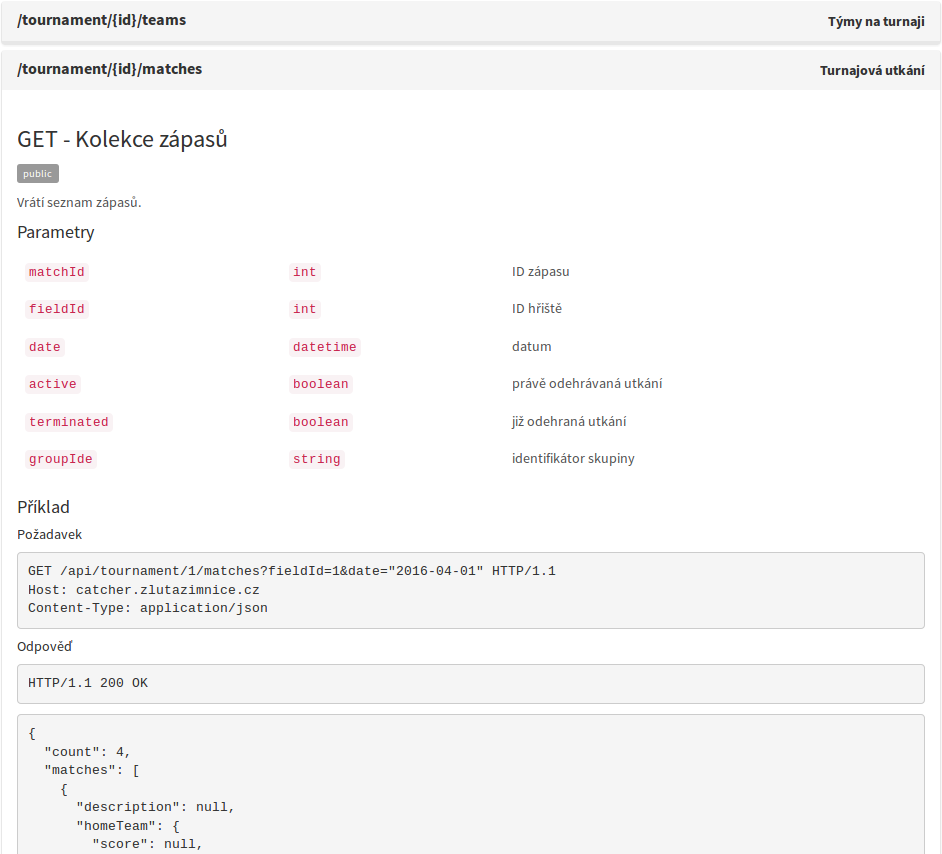
\includegraphics[width=130mm]{./images/doc.png}
\caption{Ukázka z dokumentace\label{overflow}}
\label{fig:doc}
\end{figure}

% \section{Další}

% \textit{Popíšu vybrané části systému. Například jak aplikace komunikuje s databází, nebo jak se počítají SOTG, postupy ze skupin apod. Nemám ještě dovymšlené.}

 % TODO: Zminit, ze vsechno ukladani (vetsina) probiha v transakci